\section{Reciprocally Inconsistent Distributed Edges}
\label{sec:db-corruption}

Suppose that the edge \texttt{(a)-[:\textcolor{green}{WROTE}]->(b)} is a distributed edge, with vertices \emph{a} and \emph{b} in servers $S_i$ and $S_j , j\neq i$,  respectively.
When a transaction writes this edge $ab$,
\begin{enumerate}
\item two writes are performed: reciprocal entries in the adjacency lists of both \emph{a} and \emph{b} are updated, and
\item write order is unconstrained: a transaction is equally likely to write \emph{a} then \emph{b} as it is to write \emph{b} then \emph{a}.
\end{enumerate}

Concurrent transactions $T_x$ and $T_y$ can interleave in the following three ways and each one is depicted in Fig \ref{fig:conf}:
\begin{enumerate}[(a)]
\item $T_x$ starts before $T_y$; it writes $a$ at $S_i$ first and then proceeds to $S_j$ across the network; $T_y$ operates the other way round, beginning with $S_j$ and proceeding to $S_i$ (see Fig \ref{fig:a}). The net effect is:  $T_x \rightarrow T_y$ at $S_i$ and at  $T_y \rightarrow T_x$ at $S_j$, where  $T \rightarrow T'$ at $S$ denotes that $T$ \emph{precedes} $T'$ at server $S$.
\item Same as the previous case, except that $T_y$ starts earlier than $T_x$ (see Fig \ref{fig:b}).
\item Same net effect as in previous two cases, except that both $T_x$ and $T_y$ start their first writes at $S_i$, $T_x \rightarrow T_y$, but $T_y$ overtakes $T_x$ in reaching $S_j$ where $T_y \rightarrow T_x$ (see Fig \ref{fig:c}).
\end{enumerate}

We could envisage three more corresponding cases (a') - (c') where the roles of $T_x$ and $T_y$ in cases (a) - (c) are simply interchanged; e.g., in case (a'), $T_y$ starts before $T_x$, writes $a$ at $S_i$ first and then proceeds to $S_j$ across the network; $T_x$ operates the other way round, beginning with $S_j$ and proceeding to $S_i$. Thus, there are only 6 ways concurrent $T_x$ and $T_y$ can interleave. The arguments we make based on cases (a) - (c) of Fig \ref{fig:conf} equally apply, by symmetry, to cases (a') - (c') and so, for brevity, we will not consider the latter.

At the end of each case in Fig \ref{fig:conf}, the last update on $a$ is by $T_y$ and that on $b$ is by $T_x$. Unless updates of $T_x$ and $T_y$ are commutative, $ab$ cannot be reciprocally consistent. As an example, suppose that $T_x$ deletes the \emph{wrote} edge while $T_y$ concurrently appends a property \emph{year}:
\begin{Verbatim}[commandchars=\\\{\},fontsize=\small,xleftmargin=.2in]
\textcolor{grey}{// Tx}
\textcolor{blue}{MATCH} (a:\textcolor{green}{Person})-[w:\textcolor{green}{WROTE}]->(b:\textcolor{green}{Book})
\textcolor{blue}{WHERE} a.\textcolor{red}{name} = 'Tolkien' \textcolor{blue}{AND} b.\textcolor{red}{title} = 'The Hobbit'
\textcolor{blue}{DELETE} w

\textcolor{grey}{// Ty}
\textcolor{blue}{MATCH} (a:\textcolor{green}{Person})-[w:\textcolor{green}{WROTE}]->(b:\textcolor{green}{Book})
\textcolor{blue}{WHERE} a.\textcolor{red}{name} = 'Tolkien' \textcolor{blue}{AND} b.\textcolor{red}{title} = 'The Hobbit'
\textcolor{blue}{SET} w.\textcolor{red}{year} = 1937
\end{Verbatim}
\begin{figure}[htp]
  \centering
  \begin{subfigure}{\linewidth}
    \centering
    \begin{tikzpicture}[node distance=2.2cm]
    \node (rect)  [draw,rounded corners,minimum width=3.5cm,minimum height=4cm,label=above:{$S_i$}] {};
  \node (rect)  [draw,rounded corners,minimum width=3.5cm,minimum height=4cm,label=above:{$S_j$},xshift=5.6cm] {};
  \node (v1) [big_vertex,xshift=0cm,yshift=0cm] {\small{\texttt{a:\textcolor{green}{Person}}}};

  \node (v2) [big_vertex,xshift=5.6cm,yshift=0cm] {\small{\texttt{b:\textcolor{green}{Book}}}};

  \node [below of=v1,yshift=1cm] {\small{\texttt{\textcolor{red}{name}:Tolkien}}};
  \node [below of=v2,yshift=1cm] {\small{\texttt{\textcolor{red}{title}:The Hobbit}}};

  \draw [thick,dashed,->,>=stealth] (0.9,0)  -- node [midway,above] {:\textcolor{green}{\small{\texttt{WROTE}}}} node [midway,below,xshift=0.1cm] {\small{\texttt{\textcolor{red}{year}:1937}}} (2.7,0);
\end{tikzpicture}

    \caption{Half-corrupted edge.}
    \label{hc-edge}
  \end{subfigure}
  %
  \begin{subfigure}{\linewidth}
    \vspace{2ex}
    \centering
        \begin{tikzpicture}[node distance=2cm,scale=0.6,every node/.style={transform shape}]

      \record(
      0,
      \small{\texttt{a:Person}},
      \small{\texttt{name:Tolkien}},
      $\boldsymbol{\rightarrow}$ \textbf{\small{\texttt{wrote b}}},
      \texttt{edge},
      \texttt{edge}
      );

      \record(
      -1,
      \small{\texttt{b:Book}},
      \small{\texttt{\texttt{year:1937}}},
      \small{\texttt{title:The \hspace{-0.15cm} Hobbit}},
      ,
      \texttt{edge}
      );

      \record(-2,
      \small{\texttt{vertex id}},
      \texttt{property},
      \texttt{property},
      \texttt{edge},
      \texttt{edge}
      );

      \spaceRecord(-2.7)

      \record(-3.6,
      \small{\texttt{vertex id}},
      \texttt{property},
      \texttt{edge},
      \texttt{edge},
      \texttt{edge}
      );

    \end{tikzpicture}

    \caption{Database records.}
    \label{hc-db-rep}
  \end{subfigure}%
  \caption{Logical and storage layer representation of a half-corrupted edge.}
  \label{hc}
\end{figure}
The interleaving patterns depicted in Fig \ref{fig:conf} leave $ab$ reciprocally inconsistent, as shown in Fig \ref{hc}.

When $T_x$ and $T_y$ do not interleave,  either $T_y \rightarrow T_x$ or $T_x \rightarrow T_y$ holds at both servers $S_i$ and $S_j$; in that case, the last update on \emph{both} $a$ and $b$ would be by either $T_x$ or $T_y$, respectively. That is, when transactions update at both ends of $ab$  in \emph{some} arbitrarily chosen but identical order, $ab$ is left  reciprocally consistent after each transaction's update.

When interleaving updates leave $ab$ reciprocally inconsistent, $ab$ can be said to have become \emph{half-corrupted} because if $T_y \rightarrow T_x$ is the chosen order between $T_y$ and $T_x$, then the edge pointer in $b$ of $ab$ is in error; otherwise, the edge pointer in $a$ is erroneous. Thus, a reciprocally inconsistent edge $ab$ certainly has a corrupt half but the question of which half is corrupt has been left open.

Suppose that a future transaction $T_w$ \emph{first} reads the edge pointer of reciprocally in consistent $ab$, say, at vertex $a$. (Note that when $T_w$ reads any edge, it does not check for reciprocally consistency). At that moment, $T_w$ (implicitly) chooses the order $T_x \rightarrow T_y$ and thereby invalidates the other order $T_y \rightarrow T_x$ that prevails at vertex $b$. Thus, from that moment onward, the $b$ end of edge $ab$ becomes the corrupt end.

If no transaction ever reads the edge pointer at vertex $b$, then the order $T_x \rightarrow T_y$ effectively prevails and the half-corruption of $ab$ remains invisible to the rest of the database. However, if $T_z$ is to subsequently read the edge pointer at $b$ and write another edge based on what it read, i.e., The Hobbit has unknown author, then it is introducing updates not consistent with what $T_w$ read earlier; it thus introduces \emph{semantic corruption} into the database. Further writes based on reading semantically corrupt data also spread corruption.

A database is said to be \emph{operationally corrupt} when a significant proportion of its data records are in a semantically corrupt state. As stated earlier, we had shown that 10\%  of a distributed graph database can become semantically corrupt well within the system lifetime itself (\cite{Ezhilchelvan2018}, \cite{Webber2019}).

Two more relevant remarks on past works:
a half-corrupted edge is due to a \emph{dirty write} (ANSI \emph{P0} \cite{Berenson1995}, Adya \emph{G0} \cite{Adya2000}) in the context of distributed graph databases. If the database provides the ANSI isolation level \emph{Read Uncommitted}, it will identically order the writes of concurrent transactions and this would prevent all interleaving patterns shown in Fig \ref{fig:conf} and thus avert half-corruption altogether.
